\section{Ordered sets}
\mybox{有序集}

\begin{mydef}\label{mydef:1.5}
    Let $S$ be a set. 
    An \myKeywordblue{order} on $S$ is a relation, denoted by $<$,
    with the following two properties:
    \begin{asparaenum}[(i)]
        \item If $x\in S$ and $y\in S$ then one and only one of the statements
        \begin{equation*}
            x<y, \quad
            x=y, \quad
            y<x
        \end{equation*}
        is true.    
        \item If $x,y,z\in S$, if $x<y$ and $y<z$, then $x<z$.
    \end{asparaenum}

    The statement $x < y$ may be read as 
    $x$ is less than $y$, or 
    $x$ is smaller than $y$, or
    $x$ precedes $y$.
    (It's often convenient to write $y>x$ in place of $x<y$)
    (less-great, smaller-bigger, precedes-succeeds)

    \mybox{form wiki,\\
    The relationship x precedes y is written $x ≺ y$.  \\
    The relation x precedes or is equal to y is written x ≼ y. \\
    The relationship x succeeds (or follows) y is written x ≻ y.  \\
    The relation x succeeds or is equal to y is written x ≽ y. \\
    ≺ $\backslash\text{prec}$  \\
    ≼ $\backslash\text{preccurlyeq}$  \\
    ≻ $\backslash\text{succ}$  \\
    ≽ $\backslash\text{succcurlyeq}$  } 

    $x\leq y$ indicates that $x<y$ or $x=y$, 
    without specifying which of these two is to hold.
    In other words, $x\leq y$ is the negation of $x>y$.
\end{mydef}


\mybox{
  偏序关系:
1. 三歧性,
2. 传递性.

建立偏序关系后, 可以使用不等式进行分析. 
在后续根据极限定义计算时, 
需要大量使用不等式分析数列和函数的极限计算结果. }

\begin{mydef}
    \label{mydef:1.6}
An \myKeywordblue{ordered set} is a set $S$ in which an order is defined.
\end{mydef}

For Example, $\Q $ is an ordered set 
if $r<s$ is defined to mean that $s-r$ is a positive rational number.

\mybox{
    存在偏序关系的集合称为有序集
$\Q , \R$ 均是有序集, 但$\mathbb{C}$ 不是有序集. }

\begin{mydef}
    \label{mydef:1.7}
    (bounded above)\\
    Suppose $S$ is an ordered set, and $E \subset S$. 
    If there exists a $\beta \in S$ 
    such that $x \leq \beta$ for every $x \in E$, 
    we say that $E$ is \myKeywordblue{bounded above}, and call
    $\beta$ an \myKeywordblue{upper bound} of $E$.

    Lower bounds are defined in the same way (with $\geq$ in place of $\leq$).
\end{mydef}

\begin{mydef}
    \label{mydef:1.8}
    (least upper bound)\\
    Suppose $S$ is an ordered set, $E \subset S$, and $E$ is bounded above.
    Suppose there exists an $a\alpha \in S$ with the following properties:
    \begin{enumerate}[(i)]
        \item $\alpha$ is an upper bound of $E$.
        \item If $\gamma <\alpha$ then $\gamma$ is not an upper bound of $E$.
    \end{enumerate}

    Then $\alpha$ is called the \myKeywordblue{least upper bound} of $E$ 
    [that there is at most one such $\alpha$ is clear from (ii)] 
    or the \myKeywordblue{supremum} of $E$, and we write
    \begin{equation*}
        \alpha = \sup E.
    \end{equation*}

    The \myKeywordblue{greatest lower bound}, or \myKeywordblue{infimum}, 
    of a set $E$ which is bounded below is defined in the same manner: The statement
    \begin{equation*}
        \alpha = \inf E
    \end{equation*}
    means that $\alpha$ is a lower bound of $E$ and 
    that no $\beta$ with $\beta > \alpha$ is a lower bound
    of $E$.
\end{mydef}
\mybox{
    从上界引出最小上界, 没有直接定义最大下界, 而是使用对称定义引出. 
    从最小上界引出的最小上界性质更为常用. Dedekind分划
}

\begin{newexample}
    \label{newexample:1.9}
    \begin{asparaenum}[(a)]
        \item Consider the set $A, B$
        \begin{equation*}
            A = \{p|p^2 < 2\},\quad
            B = \{p|p^2 > 2\}.
        \end{equation*}
        $A$ has no least upper bound in $\Q $.
        $B$ has no great lower bound in $\Q $.    
        \item If $\alpha = \sup E$ exists, $\alpha$ may be or may not be a member of $E$.
        \begin{align*}
            E_1 = \{r |r\in Q, r < 0\}\\
            E_2 = \{r |r\in Q, r \leq 0\}
        \end{align*}
        \begin{equation*}
            \sup E_1 = \sup E_2 = 0,
        \end{equation*}
        and $0\not\in E_1$, $0\in E_2$.
        \item $E = \{1/n | n = 1,2,3,...\}$. 
        Then $\sup E = 1$, which is in $E$, 
        and $\inf E = 0$, which is not in $E$.
    \end{asparaenum}
\end{newexample}

\begin{mydef}
    \label{mydef:1.10}
    {\color{red}{least-upper-bound property}}\\
    An ordered set $S$ is said to have the \myKeywordblue{least-upper-bound property} 
    if the following is true:\\
    If $E \subset S$, $E$ is not empty, and $E$ is bounded above, then $\sup E$ exists in $S$.
\end{mydef}

Example \ref{newexample:1.9}(a) shows that $\Q $ does not have the least-upper-bound property.

We shall now show that 
there is a close relation between greatest lower bounds and least upper bounds, 
and that every ordered set with the least-upper-bound property 
also has the greatest-lower-bound property.

\mybox{最小上界性质与最大下界性质是等价的.}

\begin{thm}
    \label{thm:1.11}
    Suppose $S$ is an ordered set with the least-upper-bound property,
    $B \subset S$, $B$ is not empty, and $B$ is bounded below. 
    Let $L$ be the set of all lower bounds of $B$. 
    Then
    \begin{equation*}
        \alpha = \sup L
    \end{equation*}
    exists in $S$, and $\alpha = \inf B$.

    In particular, $\inf B$ exists in $S$.
\end{thm}

\begin{proof}
    Since $B$ is bounded below, $L$ is not empty. 
    Since $L$ consists of exactly those $y \in S$ 
    which satisfy the inequality $y \leq x$ for every $x \in B$, 
    we see that \myKeywordblue{every} $x \in B$ \myKeywordblue{is an upper bound of} $L$. 
    Thus $L$ is bounded above.
    Our hypothesis about $S$ implies therefore that 
    $L$ has a supremum in $S$; 
    call it $\alpha$.

    If $\gamma < \alpha$ then (see Definition \ref{mydef:1.8}) 
    $\gamma$ is not an upper bound of $L$, 
    hence $\gamma \not\in B$. 
    It follows that $\alpha \leq x$ for every $x \in B$. 
    Thus $\alpha \in L$.

    If $\alpha < \beta$ then $\beta \not\in L$, 
    since $\alpha$ is an upper bound of $L$.

    We have shown that $\alpha \in L$ 
    but $\beta \not\in  L$ if $\beta > \alpha$. 
    In other words, $\alpha$ is a lower bound of $B$, 
    but $\alpha$ is not if $\beta > \alpha$. 
    This means that $\alpha = \inf B$.
\end{proof}

\mybox{% mynotes
这个证明第一次看比较难理清\\
我试着用自己的话重写梳理一下:
已知条件
$S$, ordered set + least-upper-bound property.
$B\in S$, $B\neq \varnothing $, $B$ is bounded below.
$L$ is the set of all lower bounds of $B$.
$\exists \alpha\in S$, $\alpha = \sup L$, and $\alpha = \inf B$.}

\begin{proof}
    % proof:
    思路 由最小上界 $\Rightarrow $ 最大下界
    % \begin{equation*}
    %     \begin{array}{ccc}
    %         \text{最小上界}  & \rightarrow  &\text{最大下界} \\
    %         \downarrow      &               &\uparrow \\
    %         L\text{最小上界}  & \rightarrow  &B\text{最大下界} \\
    %     \end{array}
    % \end{equation*}
    \begin{figure}[htbp]
        \centering
        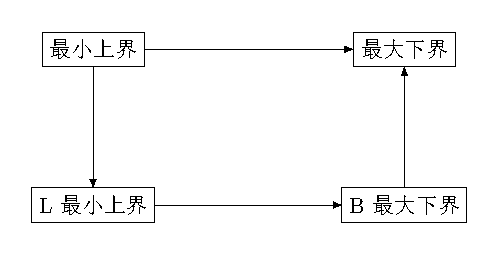
\includegraphics[width=0.7\linewidth]{pic/chap01sec02_proof11.pdf}
        % \caption{function-mapping}
        \label{fig:chap01sec02_proof11}
    \end{figure}

    $L = \{y| y\in S; \forall x\in B, y\leq x\}$
    关于 $L$ 中有没有不在 $S$ 中的元素这一点我还没想明白.
    定理中只是说 $L$ 是 $B$ 的下界组成的. 
    $B$ 是 $S$ 的子集, 但 $B$ 的下界不一定全在 $S$ 中. 

    $L$ 由 $B$ 在 $S$ 中的全部下界组成

    $\forall x\in B$, $x$ 为 $L$ 的上界. $L\subset S$.
    $S$ 有最小上界性质,
    $\therefore \exists \alpha\in S$, $\alpha = \sup L$.

    $\forall \gamma <\alpha$ 由 $\alpha = \sup L$ 的定义 (\ref{mydef:1.8})
    $\gamma$ 不是 $L$ 的上界.

    $\forall x \in B$, $x$ 为 $L$ 的上界, $x \geq \alpha$. $\therefore \alpha \in L$.

    $\alpha < \beta$, $\alpha = \sup L$. $\therefore \beta \not\in L$.
    $L$ 由 $B$ 在 $S$ 中的全部下界组成, $\beta \not\in L$.
    $\beta$ 不是 $B$ 的下界.

    $\therefore \alpha = \inf B$, $\inf B\in S$.
\end{proof}

